% !TEX program = pdflatex

\documentclass[a4paper]{tufte-handout}

\author{James Penn}
\title{A Shallow Water Model}


%\hypersetup{colorlinks}                               % use non-coloured hyperlinks
\usepackage{lmodern}                                  % allow arbitrary size fonts
\usepackage[utf8]{inputenc}                           % allow UTF-8 formatting of source
\usepackage[english]{babel}                           % use English typesetting rules

\usepackage{MinionPro}                                % Adobe MinionPro Serif font
\usepackage{MyriadPro}                                % Adobe MyriadPro Sans-serif font

\usepackage{booktabs}                                 % nicely typeset tabular material
\usepackage{amsmath}                                  % basic maths
\usepackage{siunitx}                                  % SI unit formatting

\usepackage{graphicx}
\setkeys{Gin}{width=\linewidth,totalheight=\textheight,keepaspectratio}
\graphicspath{{images/}} % set of paths to search for images

\usepackage{minted}

% % bibliography
% \usepackage[square, numbers]{natbib}


% JP commands
\newcommand{\vect}[1]{\ensuremath{\boldsymbol{#1}}}
\newcommand{\curly}[1]{\ensuremath{\mathrm{#1}}}
\renewcommand{\d}[1]{\ensuremath{\operatorname{d}\!{#1}}}
\newcommand{\diff}[2]{\frac{\d{} #1}{\d #2}}
\newcommand{\lagr}[1]{\frac{\operatorname{D}\! #1}{\operatorname{D}\!t}}
\newcommand{\dd}[2]{\frac{\partial #1}{\partial #2}}
\newcommand{\tensorcol}[1]{% inline column vector
  \ensuremath{\left(\begin{smallmatrix}#1\end{smallmatrix}\right)}
}
\newcommand{\minihead}[1]{\vspace{0.5 em} \noindent \textbf{#1} \vspace{0.3 em}  \\ \noindent}
\newcommand{\icode}[1]{\texttt{#1}}
\newcommand{\imag}{\mathrm{i}}  % imaginary unit i
\newcommand{\euler}{\mathrm{e}}  % Euler's constant e



\begin{document}

  \section{Introduction}
  \label{sec:Introduction}
  The Python code \texttt{linearshallowwater.py} models the linearised shallow
  water equations on the beta plane.
  These are
  \begin{align}
    \dd{u}{t} - fv &= - g \dd{h}{x} \\
    \dd{v}{t} + fu &= - g \dd{h}{y} \\
    \dd{h}{t} + H(\dd{u}{x} + \dd{v}{y}) &= 0
  \end{align}
  where fluid height $\eta = H + h$ and Coriolis parameter $f=f_0 + \beta y$.

  The partial derivatives in space are approximated by a first-order central
  difference method and timestepping is performed using a linear-multistep method,
  the three-step Adams-Bashforth method.
  Appendix A \ref{sec:appendixa} details the numerical methods used.

  \section{Experiments}
  \label{sec:Experiments}

  \subsection{Experiment 1}
  \label{sub:Experiment 1}

  \begin{itemize}
    \item Download the python script \texttt{linearshallowwater.py} from the
    course website\footnote{\url{http://empslocal.ex.ac.uk/people/staff/gv219/ecmm719/index.html}}.
    \item Set \texttt{experiment = '2d'} and run the code from the command line.
    \begin{minted}[mathescape]{bash}
      $ cd Downloads
      $ python linearshallowwater.py
    \end{minted}
    \item You should see the case for a non-rotating fluid begin to run on
    your screen.  The height field is set with an initial condition of a small
    gaussian added to one point in the field.  As the equations evolve $u$ and
    $v$ velocities are induced and the gravity waves radiate outwards.
    \begin{marginfigure}
      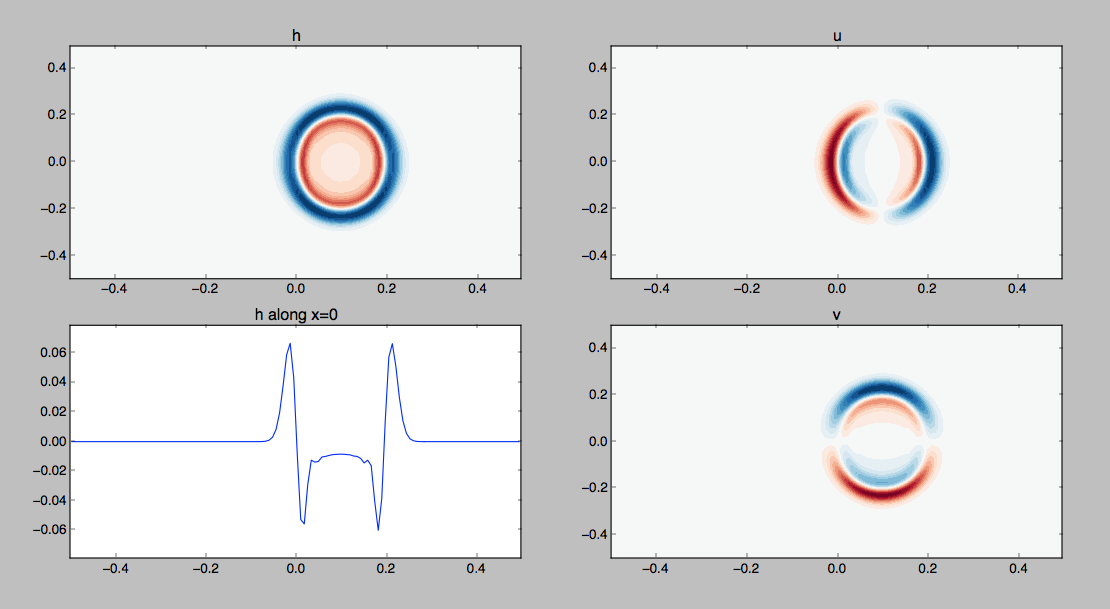
\includegraphics{gravity_waves}
      \caption{Gravity waves propagating away from an initial disturbance.}
      \label{fig:gravwaves}
    \end{marginfigure}
    \item Fin
  \end{itemize}

  \section{Appendix A: Numerics}
  \label{sec:appendixa}

  \noindent The shallow water model uses finite difference methods to calculate
  the derivatives in the spatial dimension.

  In the simplest case, the domain $x \in [-L/2, L/2]$ is split into $N$
  subdivisions, creating $N+1$ \emph{nodes} of distance $\Delta x = L/(N+1)$ apart.
  We denote the positions of the nodes $x_0, x_1, ..., x_{N+1}$ where $x_j = j \Delta x$.

  For a continuous function $u(x)$ the definition of a derivative is
  \begin{equation}
    \dd{u}{x} = \lim_{\Delta x \to 0} \frac{u(x + \Delta x) - u(x)}{\Delta x}
  \end{equation}
  For our discrete model, at the node points $x_j$ described above we denote
  the value of $u_j = u(x_j)$ and simply approximate the derivative by considering
  only values at the closest node points
  \begin{equation}
    \label{eq:cendiff}
    \dd{u_j}{x} \simeq \frac{u_{j+1} - u_{j-1}}{2 \Delta x}
  \end{equation}
  This is the \emph{central difference} method of calculating a spatial derivative
  and is used extensively in this model.
  \begin{marginfigure}
    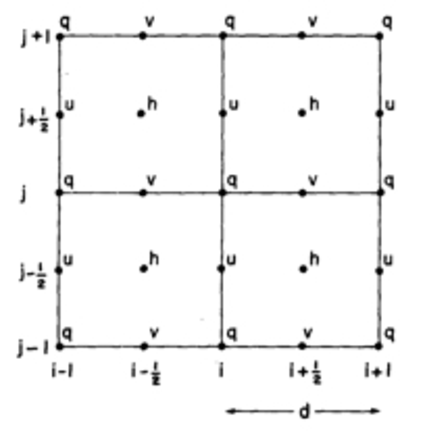
\includegraphics{cgrid}
    \caption{The Arakawa-C grid. From \citep{Arakawa:1981bx}}
    \label{fig:cgrid}
  \end{marginfigure}
  Obviously, an error has been introduced here for any function other than a
  straight line, the error is proportional to $\Delta x$.
  If $\Delta x$ is reduced ($N$ increases), error will be reduced but computing time will be
  increased as to calculate the value of $u(x)$ across the domain requires
  calculating the value at $(N+1)$ positions.
  The central-difference equation (\ref{eq:cendiff}) has a weakness - it is
  performed over a distance of $2 \Delta x$ and the new value at $u_i$ is
  decoupled from the previous value at this point as it depends solely on
  values at neighbouring nodes.

  For improved numerical stability, the locations of u, v and h values are
  staggered in a configuration known as the \emph{Arakawa-C grid} (Figure~\ref{fig:cgrid}).
  This distribution of value nodes means that, for example, the central difference
  approximation
  \begin{equation}
    \dd{h}{x} \simeq \frac{h_{i+1/2} - h_{i-1/2}}{\Delta x}
  \end{equation}
  falls at the location of the $u_i$ node.
  In the linearised shallow water equations this is a desirable property:
  the value of $u$ at the next timestep depends on $\dd{h}{x}$ and using
  the staggered configuration the dependency is on immediately adjacent values
  over a distance of $\Delta x$.

  Consider the other spatial derivative terms in the shallow water equations.
  How they can be approximated by a central difference method when using the
  Arakawa-C grid?


  In simulating the shallow water equations we are essentially solving
  an initial value problem.
  Once the spatial derviatives have been approximated the equations can
  be stepped forward in time in a similar manner to
  This idea can be extended to thinking about derivatives in time also.
  For example, the linear momentum equation can be discretised
  \begin{equation}
    \frac{u_j^{(n+1)} - u_j^{(n)}}{\Delta t} - fv_j^{(n)} = - \frac{\phi_{j+1}^{(n)} - \phi_{j-1}^{(n)}}{2 \Delta x}
  \end{equation}
  where $^{(n+1)}$ denotes the index in time in the same way $_j$ denotes
  index in space.

  This can be rearranged to calculate the value of $u_j^{(n+1)}$ entirely in
  terms of variables at the $^{(n)}$ time-level.
  \begin{equation}
    u_j^{(n+1)} = u_j^{(n)} + {\Delta t}
      \left( fv_j^{(n)} - \frac{\phi_{j+1}^{(n)} - \phi_{j-1}^{(n)}}{2 \Delta x} \right)
  \end{equation}
  Timestepping in this manner is known as \emph{Euler's method}.
  This is an \emph{explicit} numerical scheme as the value at time $^{(n+1)}$
  depends solely on values at $^{(n)}$.

  Euler's method is the simplest possible timestepping procedure,
  for better accuracy here the slightly more complicated three-step \emph{Adams-Bashforth}
  method is used for timestepping.  Adams-Bashforth $n$-step routines are a family
  of \emph{linear multistep} methods that calculate the state at the next timestep
  based on a weighted average of the states at the previous $n$ time levels.

  For a differential equation of the form $ \diff{y}{t} = f(t, y) $ the
  first three Adams-Bashforth multistep methods are
  \begin{align*}
    y_{n+1} &= y_n + \Delta t f(t_n, y_n)  \\
    y_{n+2} &= y_{n+1} + \Delta t \left( \frac{3}{2}f(t_{n+1}, y_{n+1}) - \frac{1}{2}f(t_n, y_n) \right) \\
    y_{n+3} &= y_{n+2} + \Delta t \left( \frac{23}{12} f(t_{n+2}, y_{n+2}) - \frac{4}{3} f(t_{n+1}, y_{n+1}) + \frac{5}{12}f(t_n, y_n)\right) \\
  \end{align*}
  For a comprehensive (and rigorous!) discussion of numerical methods in
  geophysical fluids problems see Dale Durran's book \cite{Durran:2010hy}.


\bibliography{biblio}
\bibliographystyle{plainnat}

\end{document}
